\chapter{Análisis}
\label{cap:analisis}

En este capitulo se detalla los diferentes análisis realizados para poder implementar los métodos de \textit{self-calibration} y \textit{Bispectrum}, de tal manera de obtener una buen resultado de estos métodos. 

\section{Pyralysis}

Un aspecto importante para el desarrollo de los métodos \textit{Bispectrum} y \textit{Self-calibration} es el formato de los datos a trabajar. Los conjuntos de datos utilizados vienen en formato \textit{measurement set} (MS) que permite el almacenamiento de visibilidades en tablas \citep{kemball2000measurementset},  el cual extiende el formato AIPS++ definido por \cite{cornwell1997design} que almacenaba los datos generados a través de clases en el lenguaje C++. No obstante, el formato a trabajar es el entregado por el framework Pyralysis, el cual lee el conjunto de datos en su formato MS y lo transforma a un objeto de Pyralysis. Este permite un fácil acceso a información relevante, como las visibilidades observadas y modelo, las antenas asociadas a estas, el tiempo de medición, los pesos, entre otros datos. De esta manera, se debe tener en consideración el formato de Pyralysis ya que los métodos de \textit{Bispectrum} y \textit{self-calibration} se deben implementar dentro de este framework.

Como se menciona en la sección \ref{subsec:pyralysis}, Pyralysis es un framework que utiliza la programación orientada a objetos, por lo que los datos y funcionalidades de este son accesibles a través de clases que contienen atributos y métodos. Estas clases son importantes a considerar para la implementación de los métodos de \textit{self-calibration} y \textit{Bispectrum} debido a que se utilizarán en conjunto con las nuevas clases necesarias para la implementación de los métodos antes mencionados. 

\begin{itemize}
    \item \textbf{DaskMS}: Clase de I/O que permite el manejo de los conjuntos de datos en su formato MS, además de su escritura y lectura. 
    \item \textbf{Dataset}: Clase que representa el conjunto de datos ingresado. Permite el acceso a datos como antenas, líneas base, polarizaciones, campos, observaciones y subms.  
    \item \textbf{SubMS}: Subdivisión del conjunto de datos debido a que \verb|dask-ms| particiona según los \textit{fields} y \textit{spectral windows}. Permite el acceso a las visibilidades. 
    \item \textbf{VisibilitySet}: Representa las visibilidades para la partición de el conjunto de datos. Permite el acceso a datos como las visibilidades observadas y modelo, pesos, antenas asociadas a las visibilidades, tiempo, \textit{scan number}, entre otros. 
    \item \textbf{Fits}: Clase de I/O que permite el manejo de archivos de tipo FITS.
    \item \textbf{Image}: Clase que representa una Imagen. 
    \item \textbf{ModelVisibilities}: Clase que permite agregar la columna modelo a partir de una imagen ingresada.  
    \item \textbf{ObjectiveFunction}: Clase que representa una función objetivo. Esta permite calcular el valor de la función y también el valor de su gradiente. 
    \item \textbf{Transformer}: Clase que representa un transformador general, donde su implementación especifica debe realizar un cambio en el conjunto de datos ingresado.
\end{itemize}

Entre las clases listadas anteriormente se encuentran aquellas que permiten acceder a la información del conjunto de datos, que si bien son de fácil acceso hay que tener en consideración el como están almacenadas. Un aspecto importante son las dimensiones para cada uno de los datos, ya que los cálculos a realizar se deben hacer con las dimensiones correctas. Por esto mismo en la tabla \ref{tab:shapes} se mencionan las dimensiones de los datos a utilizar. 

\begin{table}[!ht]
	\begin{center}
		\caption{Tabla con dimensiones de datos en Pyralysis}
		\begin{tabular}{| c | c |}
			\hline
			Dato & Dimensiones\\ \hline
			Visibilidades & (row, channel, correlation)\\ \hline
            Pesos & (row, correlation)\\ \hline
            Antena & (row) \\ \hline
            Tiempo & (row)\\ \hline
            UVW &  (row, uvw)\\ \hline
            Flags &  (row, channel, correlation)\\ \hline
		\end{tabular}
		\label{tab:shapes}
	\end{center}
	\begin{center}
		Fuente: Elaboración propia.
	\end{center}
\end{table}

\section{\textit{Self-calibration}}

%EXPLICAR TEMA DE OPTIMIZACIÓN

Un parámetro a considerar en la implementación de \textit{self-calibration} es el rango de tiempo en el cual se quiere realizar este método, es decir, en grupos de observaciones que se hayan realizado dentro de un tiempo determinado. Para esto el conjunto de datos debe venir ordenado crecientemente en el tiempo, de tal manera que el agrupamiento de los datos por rango se realice de manera efectiva. En la Figura \ref{fig:time_vs_row} se observa como es el comportamiento del tiempo para un conjunto de datos. 

\begin{figure}[!ht]
	\centering
	\captionsetup{justification=centering}
	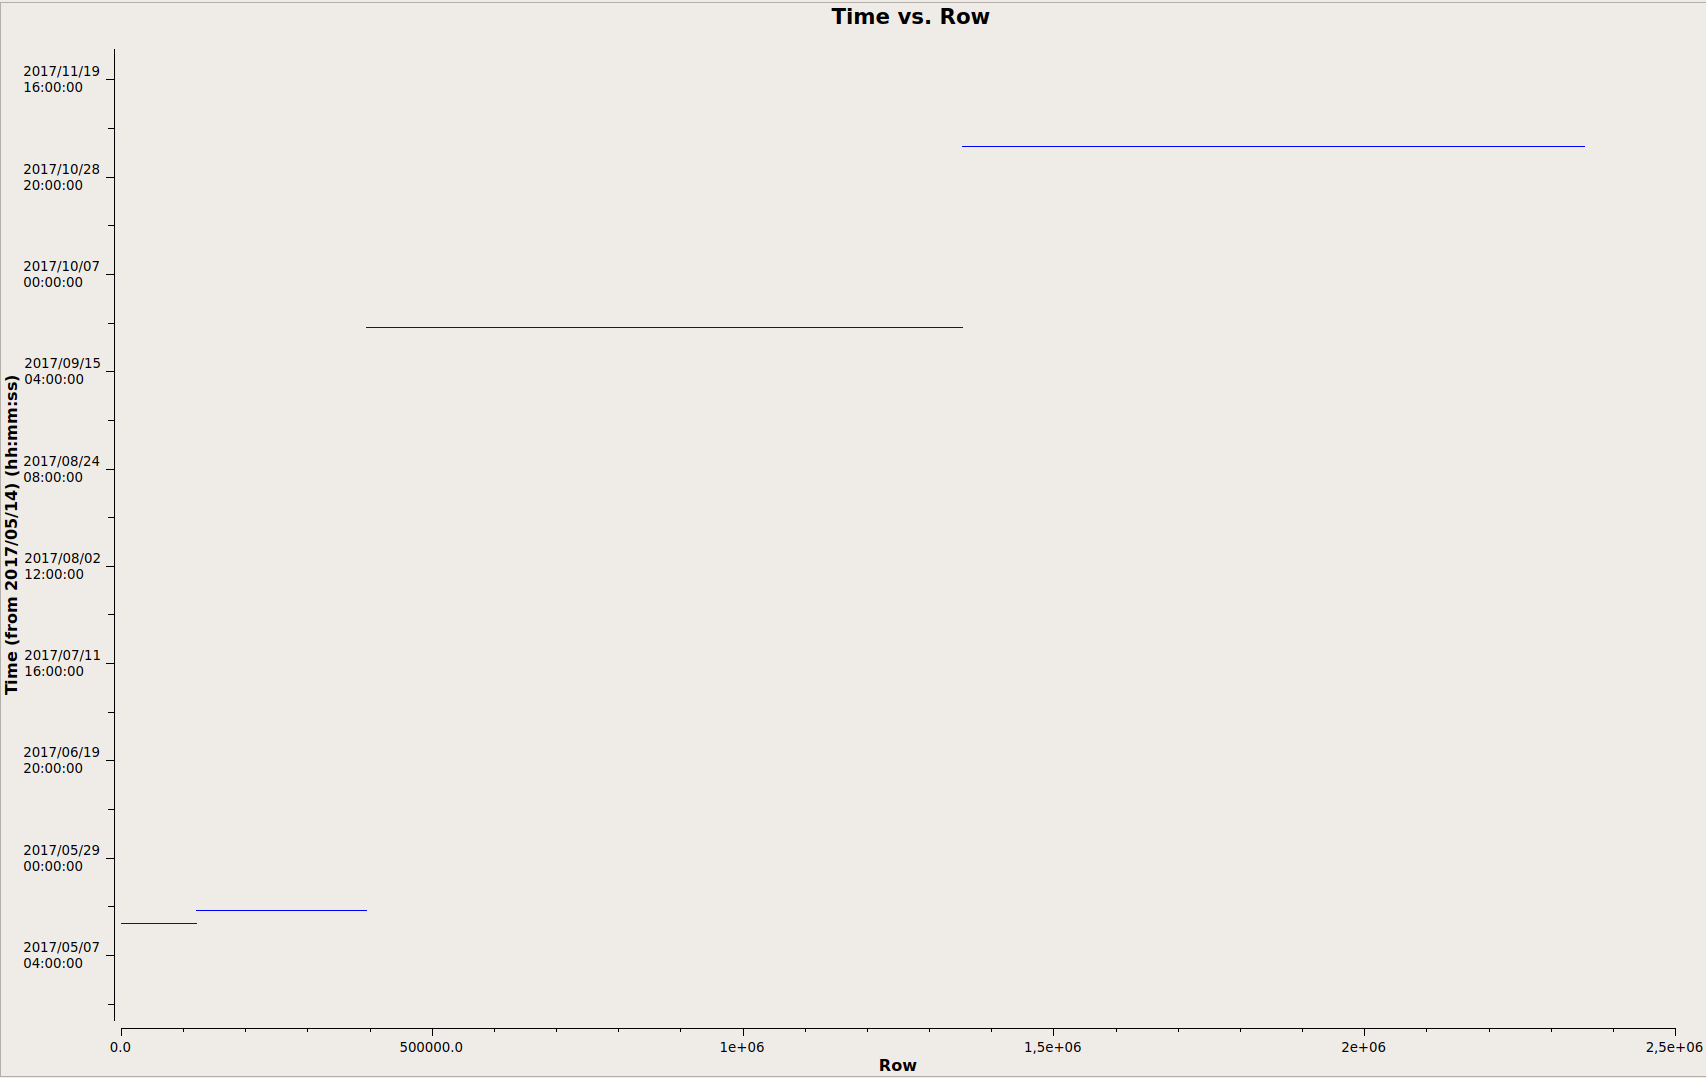
\includegraphics[scale=0.3]{images/time_vs_row.png}
	\caption[Tiempo de medición para GWLup]{Tiempo de medición para GWLup. Fuente: Elaboración propia}
	\label{fig:time_vs_row}
\end{figure}

Como se observa el tiempo aumenta pero se puede llegar a presentar ciertos cortes en los datos, esto debido al cambio de fecha de cuando se capturaron. Teniendo en cuenta esto se crea un algoritmo que agrupa los datos que estén dentro de un mismo rango de tiempo, pero en caso de presentarse un salto de tiempo como se menciona anteriormente, este no presentará un mayor problema debido a que si el rango de tiempo es lo bastante grande, el corte entrará dentro de los datos agrupados. 

El algoritmo necesita los tiempo en que fueron capturado los datos y el rango de tiempo deseado para agruparlos. La forma de realizar esto se muestra en el algoritmo \ref{alg:get_index}, donde inicialmente se define la diferencia de los tiempos para ser recorridas y un índice (denominado índice actual) que indica desde que lugar comienza y un índice final que indica en que parte termina el conjunto de datos agrupado. Luego de esto se itera hasta que el índice definido alcance el final del arreglo de las diferencias de tiempo, donde en cada iteración se ve hasta que punto los datos entran dentro del rango de tiempo y se define este límite como un índice final que será agregado a una lista de índices, además de hacer cero todos los datos que estén dentro del grupo para que no vuelvan a ser considerados. Para definir el siguiente valor del índice inicial que se evalúa en cada iteración se tienen 3 casos.

\begin{enumerate}
    \item El índice actual es igual al índice final, que es cuando solo un dato entra en el grupo, por lo que el índice actual será igual al índice final mas uno. 
    \item El índice final es igual a cero, o que quiere decir que se alcanza el final del arreglo por lo que el índice actual será igual al largo del arreglo de la diferencia de tiempos. 
    \item No se cumple ningún caso anterior por lo que el índice actual será igual al índice final. 
\end{enumerate}


\begin{algorithm}[!ht]
	\caption{Algoritmo de partición de tiempo.}
	\label{alg:get_index}
	\begin{algorithmic}[1]
	\REQUIRE Tiempo, rango de tiempo.
	\ENSURE Índices de corte. 	
	\STATE $timeDiff \gets diff(time)$
        \STATE $actualIndex  \gets 0$
        \STATE $indexList \gets [0]$

        \WHILE{$actualIndex \leq len(timeDiff) - 1$} 
            \STATE{$endIndex = (cumsum(timeDiff) \leq timeRange).argmin()$} 
            \IF {$actualIndex == endIndex$}
                \STATE $actualIndex = endIndex + 1$
            \ELSIF{$endIndex == 0$}
                \STATE $actualIndex = len(timeDiff)$
            \ELSE
                \STATE $actualIndex = endIndex$
            \ENDIF   
            \STATE $indexList.append(actualIndex)$
            \STATE $timeDiff[:actualIndex] = 0$
        \ENDWHILE 
	\RETURN $indexList$
	
	\end{algorithmic}
\end{algorithm}

En cuanto al algoritmo de \textit{self-calibration}, se debe tener en cuenta lo mencionado en optimizar la ecuación \ref{eq:self-calibration}, sin embargo en diversas implementaciones, como gaincal de CASA \citep{gaincal_task} y rascil \citep{rascil}, utilizan una variación de división de las visibilidades observadas por las modelo para encontrar el valor de las ganancias. De esta manera, se propone explorar este enfoque para el \textit{self-calibration} a implementar, donde para esto se debe tener en consideración la ecuación \ref{eq:self-calibration-3} que permite relacionar las ganancias con las visibilidades observadas y modelo, donde esta permite obtener las ganancias para la fase como amplitud.

\begin{equation}
        \sum |V_{ij} - g_{i}g_{j}^{*}\tilde{V}_{ij}|^2
        \label{eq:self-calibration}
\end{equation}

\begin{equation}
    V_{i,j,corr} = \frac{\tilde{V}_{ij}}{g_{i}g_{j}^{*}}
    \label{eq:self-calibration-3}
\end{equation}

\subsection{Fase}

Para corregir la fase con \textit{Self-calibration} es necesario comprender que las ganancias se pueden definir como indica la ecuación \ref{equation:gains}, donde el gran interés se encuentra en encontrar los ángulos ($\theta$) por pares de antenas que deben ser aplicados para corregir la fase que afecta a las visibilidades. Para esto es necesario definir la \ref{eq:self-calibration-3} junto con la expresión completa de las ganancias (ecuación \ref{equation:gains}), obteniendo así la ecuación \ref{eq:self_inicial}. 

\begin{equation}
    g_{i}g_{j}^{*} = e^{2\pi i|\theta_{i} - \theta_{j}|}
    \label{equation:gains}
\end{equation}

\begin{equation}
    V_{i,j,corr} = \frac{\tilde{V}_{ij}}{e^{2\pi i|\theta_{i} - \theta_{j}|}}
    \label{eq:self_inicial}
\end{equation}

Es posible obtener el valor para un $\theta$ asociado a una antena $i$ al comenzar a realizar operaciones sobre la ecuación \ref{eq:self_inicial}, de tal manera de dejar $\theta$ despejado. Para esto se presentan a continuación las operaciones aritméticas realizadas, partiendo por un despeje simple sobre la ecuación \ref{eq:self_inicial} dando como resultado la ecuación \ref{eq:phase1}. 

\begin{equation}
    e^{2\pi i|\theta_{i} - \theta_{j}|}= \frac{\tilde{V}_{ij}}{V_{i,j,corr}}
    \label{eq:phase1}
\end{equation}

Aún así en la ecuación \ref{eq:phase1} se tienen dos ángulos distintos ($\theta_{i}, \theta_{j}$), lo que se consideraría las incógnitas a encontrar, sin embargo se tendría dos incógnitas y una ecuación por lo que no es posible encontrar el valor para ambos ángulos. Por lo mismo, para solventar esa complicación se asume que una antena tendrá ganancia 0 y se le define como antena de referencia, por lo que solo se trabajan con visibilidades que tengan asociada esta antena. Esto permite que en la ecuación \ref{eq:phase1} desaparezca un ángulo transformándose así a la ecuación \ref{eq:phase2}.

\begin{equation}
    e^{2\pi i|\theta_{i}|}= \frac{\tilde{V}_{ij}}{V_{i,j,corr}}
    \label{eq:phase2}
\end{equation}

Como se muestra en la ecuación \ref{eq:phase3}, las ganancias pueden ser divididas en coordenadas polares y cartesianas. Esto trae consigo una ventaja ya que nos permite relacionarla con la tangente mediante la ecuación \ref{eq:phase4}, permitiendo así eliminar las amplitudes que afectan a la parte imaginaria como real. 

\begin{equation}
    e^{2\pi i|\theta_{i}|} =  cos(2 \pi \theta_i) + i  sen(2 \pi \theta_i) 
    \label{eq:phase3}
\end{equation}

\begin{align} 
Re = cos(2 \pi \theta)\\ 
Im = sen(2 \pi \theta)
\end{align}


\begin{equation}
    tg(2\pi \theta_i) = \frac{Im}{Re}
    \label{eq:phase4}
\end{equation}

Finalmente, la ecuación que permite obtener el ángulo que se debe aplicar para corregir esta dada por la ecuación \ref{eq:phase5}.

\begin{equation}
    \theta_{i} = \frac{1}{2\pi}arctg(\frac{Im}{Re})
    \label{eq:phase5}
\end{equation}

Todo lo mencionado anteriormente es combinado en un algoritmo en el cual se obtiene los ángulos para las visibilidades asociadas a la antena de referencia, se calcula los rangos de tiempo y para cada rango se realiza el promedio ponderado reemplazando los nuevos ángulos. Este se puede ver representado en el algoritmo \ref{alg:selfcalibration-impl}. Cabe destacar que dentro de este algoritmo se representa el algoritmo \ref{alg:get_index} por la función \textit{get\_index} y por otro lado la función \textit{get\_thetas} aplica la ecuación \ref{eq:phase5} mostrada anteriormente. 

\begin{algorithm}[!ht]
	\caption{Algoritmo de \textit{Self-calibration} implementado}
	\label{alg:selfcalibration-impl}
	\begin{algorithmic}[1]
	\REQUIRE Dataset en formato MS, rango de tiempo, antena de referencia.
	\ENSURE Dataset en formato MS.
	
	\FOR{$spectral\ window$}
	    \STATE $vis\_obs \gets visibilities.data$ \\
	    \STATE $vis\_mod \gets visibilities.model$ \\ 
        \STATE $weight \gets visibilities.weight$ \\
        \STATE $time \gets visibilities.time$ \\ 

        \STATE $vis\_ant\_ref \gets where(vis\_obs.antenna1 == ant\_ref\ or\ vis\_obs.antenna1 == ant\_ref)$

        \STATE $thetas \gets get\_thetas(vis\_obs, vis\_mod)$
        
        \STATE $indexs \gets get\_index(time, time\_range)$
        \FOR{ $i\ in\ len(indexs)$ }
            \STATE $slice \gets slice(indexs[i]:index[i+1])$\\

            \STATE $thetas\_ant\_ref \gets thetas[slice]$\\
            \STATE $weight\_ant\_ref \gets weight[slice]$\\

            \STATE $wheighted\_thetas \gets thetas\_ant\_ref * weight\_ant\_ref$ \\ 
            \STATE $sum\_weight \gets sum(weight\_ant\_ref)$\\
            \STATE $result \gets wheighted\_thetas / sum\_weight$\\

            \STATE $thetas[slice] \gets result$\\
        \ENDFOR 
            
        \STATE $vis\_ant\_ref \gets applycal(vis\_obs,thetas)$\\
	 
	\ENDFOR
	
	\RETURN $vis\_ant\_ref$
	
	\end{algorithmic}
\end{algorithm}

Aún así puede existir el caso donde el tiempo ingresado sea definido por 'inf', es decir, un tiempo infinito. Para solventar este caso el promedio se realiza por número de \textit{scan}, por lo que no existiría un rango de tiempo asociado sino que se promediaría por visibilidades asociadas a un \textit{scan}. La diferencia con el algoritmo \ref{alg:selfcalibration-impl} ya no estaría utilizando el algoritmo \ref{alg:get_index} y tampoco realizando la iteración por las particiones encontradas, sino que se buscaría los números de \textit{scan} asociados al conjunto de datos y se iteraría en cada uno para buscar las visibilidades asociadas para realizar el mismo promedio que se realiza en el algoritmo \ref{alg:selfcalibration-impl}.

Por otro lado, el promedio ponderado se realiza sobre los ángulos encontrados mediante la ecuación \ref{eq:phase5} y este es calculado mediante la ecuación \ref{eq:prom} que será aplicado antes de realizar el \textit{applycal}. Donde $\theta$ son los ángulos encontrados y $w$ es el peso asociado a las visibilidades asociadas a los $\theta$.

\begin{equation}
    \theta' = \frac{\sum \theta w}{\sum w}
    \label{eq:prom}
\end{equation}

La función \textit{applycal} realiza la acción de aplicar los $\theta$ encontrados a las visibilidades agrupadas, ya sea mediante rango de tiempo o \textit{scan\_number}. Para hacer esto implementa la ecuación \ref{eq:applycal}.

\begin{equation}
    V_{corr} = \frac{V_{obs}}{e^{2 \pi i \theta}}
    \label{eq:applycal}
\end{equation}

\subsection{Amplitud}

Para la realización de la calibración en amplitud se toma en consideración el análisis realizado para fase, pero la ecuación \ref{eq:phase2} se transforma en la ecuación \ref{eq:amp1}. Así también, otra diferencia a encontrar es en la función \textit{applycal} utilizada en al algoritmo \ref{alg:selfcalibration-impl}, que es dado por la ecuación \ref{eq:amp2}.

\begin{equation}
    A = \bigg|\frac{V_{obs}}{V_{mod}}\bigg| 
    \label{eq:amp1}
\end{equation}

\begin{equation}
    V_{corr} = \frac{V_{obs}}{A}
    \label{eq:amp2}
\end{equation}

Al igual que en el caso de la fase, si se ingresa un valor como 'inf' para el tiempo, se considera la utilización de las visibilidades asociadas a un número de \textit{scan} para poder realizar el promedio ponderado. 

\section{\textit{Bispectrum}}
\label{sec:bispectrum}

Para utilizar la ecuación \ref{eq:RML} mostrada en la sección \ref{subcap:sintesis} es necesario definir la ecuación a minimizar para los datos del modo bispectrum, para estos se utilizará la definida en el articulo \cite{Chael_2018}. Este define la ecuación \ref{eq:bispectrum_2}. 

\begin{equation}
    \chi^{2}_{bispec}(I) = \frac{1}{2N_{B}} \sum_{j} \frac{| V_{Bj}  - V'_{Bj}|^2}{\sigma^{2}_{Bj}}
    \label{eq:bispectrum_2}
\end{equation}

Donde $V_{Bj}$ corresponde a las visibilidades observadas de $I$ en formato \textit{Bispectrum}, $N_{B}$ corresponde a la cantidad de medidas \textit{Bispectrum}, $V'_{Bj}$ corresponde a las visibilidades observadas en formato \textit{Bispectrum} y $\sigma^{2}_{Bj}$ corresponde a la varianza estimada. Para calcular este último es necesario utilizar la ecuación \ref{eq:sigma}.

\begin{equation}
    \sigma_{B} = |V_{B}| \sqrt{\frac{\sigma^{2}_{1}}{|V_{1}|^{2}} + \frac{\sigma^{2}_{2}}{|V_{2}|^{2}} + \frac{\sigma^{2}_{3}}{|V_{3}|^{2}}}
    \label{eq:sigma}
\end{equation}

Para obtener los datos necesarios en las ecuaciones anteriores se realiza la creación de un algoritmo que busca las posibles combinaciones de tres que se pueden realizar con las antenas disponibles y calcular los pesos mediante la ecuación \ref{eq:sigma} para todos los datos. Luego de esto se busca las visibilidades observadas, modelos y los pesos relacionadas a la combinación de antenas. El algoritmo que muestra este proceso se puede ver en el algoritmo \ref{alg:bispectrum}.

Cabe destacar que se debe tener en cuenta la cantidad de antenas que tiene el conjunto de datos debido a que los números de combinaciones posibles para tríos de antenas son muchos, por ejemplo, para un observatorio como ALMA que tiene 66 antenas \citep{antenas_alma} se tendría un total de 45760 combinaciones posibles. Para esto, como se utilizó en \citet{Chael_2018}, se toma una antena de referencia que permite disminuir la cantidad de combinaciones posibles y por ende el tiempo de ejecución del método, donde si se toma el ejemplo anterior se tiene que la cantidad posible de combinaciones con una antena de referencia disminuye a 2080. 

\begin{algorithm}[!ht]
	\caption{Algoritmo de Bispectrum.}
	\label{alg:bispectrum}
	\begin{algorithmic}[1]
    \REQUIRE Conjunto de datos (MS), antena de referencia.
    \ENSURE Conjunto de datos reordenado	
    \STATE $unique\_time \gets unique(visibilities.time)$
    \STATE $antennas \gets visibilities.antenna$
    \STATE $combs \gets combination(visibilities.antennas)$
    \STATE $filt\_combs \gets [x\ for\ x\ in\ combs\ if\ ant\_ref\ in\ x]$
    \STATE $n\_comb \gets filt\_combs.size$
    \STATE $n\_utime \gets unique\_time.size$
    \STATE $nchan, ncorr \gets visibilities.shape$
    \STATE $count  \gets zeros\_like((n\_comb, n\_utime, 3, nchan, ncorr))$
    \STATE $bis\_data \gets zeros\_like((n\_comb, n\_utime, 3, nchan, ncorr))$

    \FOR{$row\ in\ visibilities$}

        \FOR{$ic, comb\ in\ filter\_combs$}
        \STATE $utime \gets unique\_time[row]$
        \STATE $antenna1 \gets antennas[row][0]$
        \STATE $antenna2 \gets antennas[row][1]$

        \IF{$antenna1 == comb[0] \ and\ antenna2 == comb[1]$}
            \STATE $bis\_data[comb, utime, 0] = visibilities[row] $
            \STATE $count[comb, utime, 0] += 1 $
        \ELSIF{$antenna1 == comb[1] \ and\ antenna2 == comb[-1]$}
            \STATE $bis\_data[comb, utime, 1] = visibilities[row] $
            \STATE $count[comb, utime, 1] += 1 $
        \ELSIF{$antenna1 == comb[0] \ and\ antenna2 == comb[-1]$}
            \STATE $bis\_data[comb, utime, 2] = visibilities[row] $
            \STATE $count[comb, utime, 2] +=  1$
        \ENDIF
    \ENDFOR

    \ENDFOR

    \STATE $bis\_data[count != 3] = 0$
    
    \RETURN $bis\_data$
	
	\end{algorithmic}
\end{algorithm}

En el algoritmo \ref{alg:bispectrum} se muestra lo implementado para el ordenamiento de los datos para luego ser calculados en el formato \textit{Bispectrum}. Inicialmente se definen las antenas y sus combinaciones de tríos filtrados por una antena de referencia, además de definir los tiempos de las visibilidades para poder ordenarlas y un contador para ver las visibilidades que cumplen con el requisito de formar un triangulo. 

Luego de definir estas variables se recorre cada visibilidad y dentro de cada iteración se recorre las combinaciones filtradas. En cada iteración para las combinaciones se verifica en que posición de la combinación está el par de antenas asociado a la visibilidad, es decir, si es $ij$, $jk$ o $ki$ y según esto se ingresa a su posición respectiva en el arreglo de datos \textit{bispectrum}, además de sumarse uno al arreglo de contador para que finalmente todas las combinaciones en que su conteo no de igual a 3 se eliminan porque sus antenas no forman un triangulo.  

El guardado de los datos en su formato \textit{Bispectrum} debe tener en consideración que la información original debe mantenerse, por lo mismo los datos calculados son almacenados en otra columna. Esta contiene unas dimensiones distintas a las visibilidades originales, donde estas son (ncomb, nutime, nant, nchan, ncorr). Cada una de estas dimensiones significa lo siguiente.

\begin{itemize}
    \item \textbf{ncomb}: Indica a que combinación de tríos de antenas pertenece las visibilidades. 
    \item \textbf{nutime}: Indica en que tiempo único se realizo la medición. Esto permite agrupar aquellas visibilidades que se obtuvieron en el mismo instante.    
    \item \textbf{nant}: Este indica a que combinación de antenas pertenece la visibilidad, es decir, si pertenece a la combinación $ij$, $jk$ ó $ki$. 
    \item \textbf{nchan}: Al igual que las visibilidades originales, este representa la cantidad de canales de las visibilidades. 
    \item \textbf{ncorr}: Al igual que las visibilidades originales, este reprenta la cantidad de correlaciones de las visibilidades.  
\end{itemize}

Sin embargo, almacenado de esta manera no se puede considerar que este en su formato \textit{Bispectrum} debido a que solo se reorganiza el conjunto de datos y no se realiza el calculo de la ecuación \ref{eq:bispectrum} para las visibilidades, ni la ecuación \ref{eq:sigma} para los pesos. La ventaja de la dimensión \texttt{nant} es que permite realizar la multiplicación en este eje de tal manera de cumplir con las ecuaciones anteriores conllevando a que la dimensión final sea (ncomb, nutime, nchan, ncorr). 

Otros datos también son guardados para complementar la información anterior, entre lo que se encuentra las antenas correspondiente al trió construido y las posiciones $uvw$ para cada visibilidad.  

\subsection{Gradiente conjugado}

Para obtener la solución necesaria para el \textit{Bispectrum} se debe implementar un método para minimizar la ecuación \ref{eq:bispectrum}, el cual para este caso se utiliza el gradiente conjugado. Para esto se calcula el gradiente de la ecuación \ref{eq:bispectrum} que está dada por la ecuación \ref{eq:derivadaBis}, donde el análisis y pasos para llegar a este están explicadas en el Apéndice \ref{finales:apendice1}.

\begin{equation}
    \begin{split}
        \frac{\partial{\chi^{2}_{bis}}}{\partial_{I_{k}}} &= \frac{-1}{N_{B}} \sum_{j} \frac{1}{\sigma^{2}_{Bj}} Re\bigg((V_{Bj} - V'_{Bj}) \bigg( \frac{\partial{V'_{Bj}}}{\partial{I_{k}}} \bigg)^{*} \bigg) \\
        &= \frac{-1}{N_{B}} \sum_{j} \frac{1}{\sigma^{2}_{Bj}} Re\bigg((V_{Bj} - V'_{Bj}) V^{'*}_{Bj} \bigg( \frac{e^{2\pi i (u_{1j}x_{k} + v_{1j}y_{k})}}{V^{'*}_{1j}} + \frac{e^{2\pi i (u_{2j}x_{k} + v_{2j}y_{k})}}{V^{'*}_{2j}} + \frac{e^{2\pi i (u_{3j}x_{k} + v_{3j}y_{k})}}{V'^{'*}_{3j}}\bigg) \bigg) 
    \end{split}
    \label{eq:derivadaBis}
\end{equation}

Un método que permite la optimización de la ecuación \ref{eq:derivadaBis} es el método del gradiente conjugado no lineal. El algoritmo \ref{alg:nolinealgradient} presenta la implementación de este método, donde se debe tener en consideración que este necesita una imagen inicial representada por $x$, un método de búsqueda lineal que es un objeto que tendrá dentro una función objetivo a minimizar, la cantidad total de iteraciones a realizar, un error asociado para el criterio de parada, un epsilon y una máscara que permite la optimización y calculo solo en un sector de la imagen. Finalmente este retorna la imagen optima encontrada. 

\begin{algorithm}[!ht]
	\caption{Algoritmo de Gradiente conjugado no lineal}
	\label{alg:nolinealgradient}
	\begin{algorithmic}[1]
	\REQUIRE Imagen, Método de búsqueda lineal, iteraciones, error, epsilon, máscara. 
	\ENSURE Gradiente de $f$. 

    \STATE $obj\_func \gets linmin.objective\_function$
    \STATE $f_{k} \gets obj\_function.calculate\_function(mask)$
    \STATE $d_{k} \gets obj\_function.calculate\_gradient(mask)$
	
	\FOR{\textit{iterations}} 
        \STATE $step \gets linmin.search(mask)$
        \STATE $x_{k+1} \gets x_{k} - step * d_{k}$
        \STATE $f_{k+1} \gets f(x_{k+1})$

        \IF{$2(f_{k+1} - f_{k}) <= error(abs(f_{k+1}) + abs(f_{k}) * epsilon)$}
         \RETURN $f'_{k+1}$
        \ENDIF

        \STATE $f_{k} \gets f_{k+1}$
        \STATE $\beta \gets rebiere\_polyak()$
        \STATE $d_{k} \gets -d_{k} + \beta d_{k-1}$
	\ENDFOR
	
	\RETURN $f'_{k+1}$
	
	\end{algorithmic}
\end{algorithm}

La búsqueda lineal es un objeto de Pyralysis que, como se mencionó anteriormente, contiene un objeto de función objetivo y permite la búsqueda del mejor paso (\textit{step}) para el gradiente. Los métodos implementados de búsqueda lineal son \textit{Backtracking} con la regla de Armijo, el método de \textit{Fixed Step} y  el método de \textit{Brent} sin embargo este último es el utilizado para las pruebas.  

El criterio de parada para el gradiente esta dada por la ecuación \ref{eq:stop_crit}. Este permite un criterio de parada más preciso sin decaer en realizar iteraciones innecesarias, además se agrega un error $\epsilon$ para evitar una división por cero. 

\begin{equation}
    \label{eq:stop_crit}
    \frac{ 2*|f_{k+1} - f_{k}|}{|f_{k+1} + f_{k}| + \epsilon}\leqslant error  
\end{equation}

Por otro lado, en la línea 12 del algoritmo \ref{alg:nolinealgradient} se menciona el calculo de un $\beta$, el cual es utilizado para obtener la nueva dirección de desplazamiento $d_{k}$. Para calcular este se utiliza el método de Polak-Ribiere-Polyak que define el valor de $\beta$ por la ecuaciíon \ref{eq:rebiere_polyak}.

\begin{equation}
    \label{eq:rebiere_polyak}
    \beta = \frac{g^{T}_{k}(g_{k} - g_{k-1})}{||g_{k-1}||^{2}}
\end{equation}


\begin{comment}
\section{Antena de referencia}

En los análisis de \textit{self-calibration} y \textit{Bispectrum} se ha mencionado el uso de una antena de referencia que ayuda de manera especifica en cada uno de los métodos. Sin embargo, una buena elección de esta es importante debido a que una mal antena seleccionada puede traer a un resultado erróneo. Lo ideal es que la antena de referencia sea una ubicada al centro del conjunto de antenas asociada al conjunto de datos.
\end{comment}


\section{Creación de datos simulados}
\label{sec:simulated_data}

Para comprobar la eficacia de los métodos implementados se necesita de un conjunto de datos controlado. Es así que se realiza la creación de un conjunto de datos simulado, o también llamado híbrido, por su combinación de información simulada y real. El proceso para esto se basa en lo propuesto en el trabajo de \citet{FernandezTesis}, por lo que se presentan aquellos aspectos que son similares. El proceso general de este es el siguiente.

\subsection{Conjunto de datos reducidos}
\label{sec:datos_reducidos}

Las alteraciones atmosféricas son variantes durante el tiempo y al ser estás las causantes de las perturbaciones en los datos se puede considerar que esta perturbación no será igual de un día para otro. Esto conlleva a que se debe disminuir el conjunto de datos a trabajar al tiempo de medición mas pequeño, de tal manera de obtener la menor variación en las perturbaciones de los datos. 

Para la creación de este conjunto de datos reducido se utiliza como inicial el obtenido a través del conjunto de datos HD163296, el cual se encuentra público en el sitio web de DSHARP. A través del uso de TaQL se puede obtener el rango de tiempo de medición junto a la cantidad de observaciones asociadas a este tiempo, de tal manera que un resumen de estos datos se puede ver en la Tabla \ref{tab:observations}. 

\begin{table}[!ht]
	\begin{center}
		\caption{Tabla con cantidad de observaciones para HD163296.}
		\begin{tabular}{| c | c | c | c | c | c |}
			\hline
			  ID observación & Fecha Inicio & Inicio & Fin & Duración & Observaciones\\ \hline
			0 & 04/06/2014 & 07:20:48 & 08:23:21 & 01:02:23 & 97522\\ \hline
            1 & 14/06/2014 & 06:30:15 & 07:32:28 & 01:02:13 & 111589\\ \hline
            2 & 16/06/2014 & 07:19:21 & 08:21:17 & 01:01:56 & 86139\\ \hline
            3 & 17/06/2014 & 07:52:13 & 08:37:14 & 00:47:01 & 58634\\ \hline
            4 & 29/06/2014 & 05:56:42 & 07:01:49 & 01:05:07 & 94778\\ \hline
            5 & 05/08/2015 & 04:34:01 & 05:43:25 & 01:29:45 & 126787\\ \hline
            6 & 08/08/2015 & 03:50:19 & 05:00:21 & 01:01:02 & 156090\\ \hline
            7 & 09/08/2015 & 01:01:41 & 02:31:28 & 01:29:47 & 50458\\ \hline
            8 & 08/09/2017 & 22:30:25 & 23:06:21 & 00:36:06 & 589711\\ \hline
            9 & 08/09/2017 & 23:29:08 & 00:27:04 & 00:57:56 & 1022112\\ \hline
		\end{tabular}
		\label{tab:observations}
	\end{center}
	\begin{center}
		Fuente: Elaboración propia.
	\end{center}
\end{table}

Si se ve los datos de la tabla \ref{tab:observations} se puede observar que la observación con id 8 la cual tiene una duración de 36 minutos con 6 segundos y un total de observaciones de 589711, es la apropiada para reducir el conjunto de datos debido a que tiene la ventana de tiempo mas pequeña y las variaciones en las perturbaciones de esta no deberían ser muy significativas. De esta manera el nuevo conjunto de datos a crear será seleccionando las visibilidades asociadas a la observación seleccionada. 

Sin embargo, la observación elegida anteriormente corresponde a aquellas capturadas a través de \textit{long-baseline} por lo que es necesario la creación de un conjunto de datos capturados a través de \textit{short-baseline}. Para esto se utiliza el mismo conjunto de datos HD163296 y se debe tener en consideración que de la tabla \ref{tab:observations} las observaciones con id desde 0 a 7 corresponden a \textit{short-baseline} y las otras corresponden a \textit{long-baseline}. De esta manera se realiza la elección de la observación con id 3, que tuvo una duración de 47 minutos con 1 segundo y contiene 85139 visibilidades, debido a que su ventana de tiempo es la mas corta. 


\subsection{Imagen sucia a conjunto de datos reducido}
\label{subsec:dirty_image}

Obtenido el nuevo conjunto de datos reducido se puede crear la imagen sucia de este que servirá para procesos posteriores. Esta se crea a través de \texttt{tclean} ofrecido por el framework CASA donde el resultado final para la observación con \textit{long-baseline} puede verse en la Figura \ref{fig:hd163296_obs8} y la observación con \textit{short-baseline} puede ser vista en la Figura \ref{fig:hd163296_obs3}. 

\begin{figure}[!ht]
 \centering
  \subfloat[Colores originales]{
   \label{fig:original_color}
    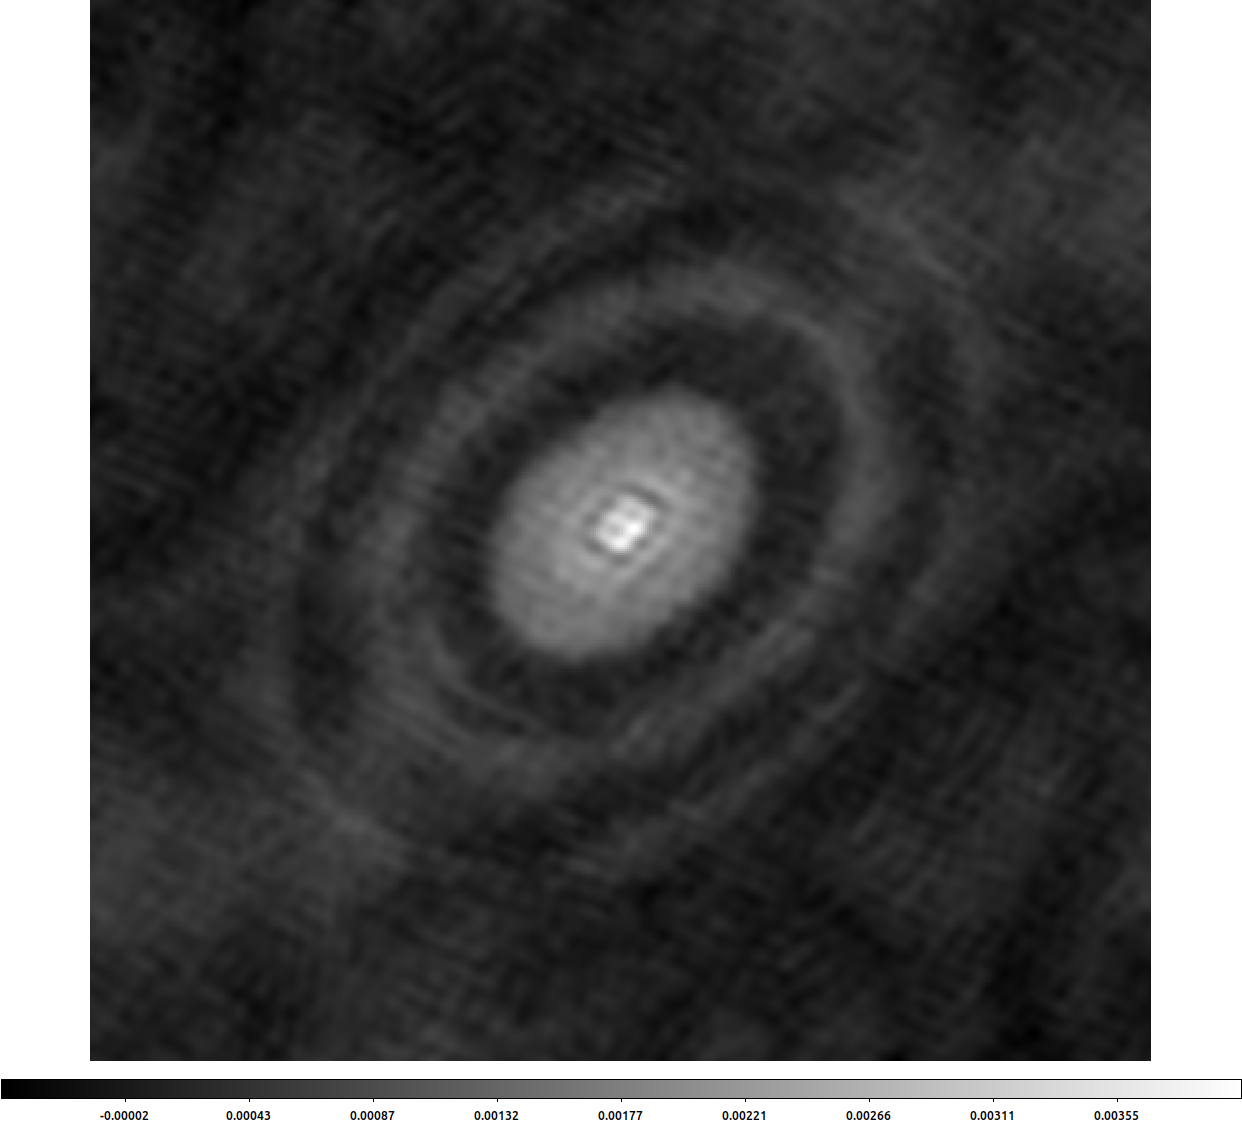
\includegraphics[width=0.45\textwidth]{images/HD163296_short8.png}}
  \subfloat[Colores artificiales]{
   \label{fig:sim_color}
    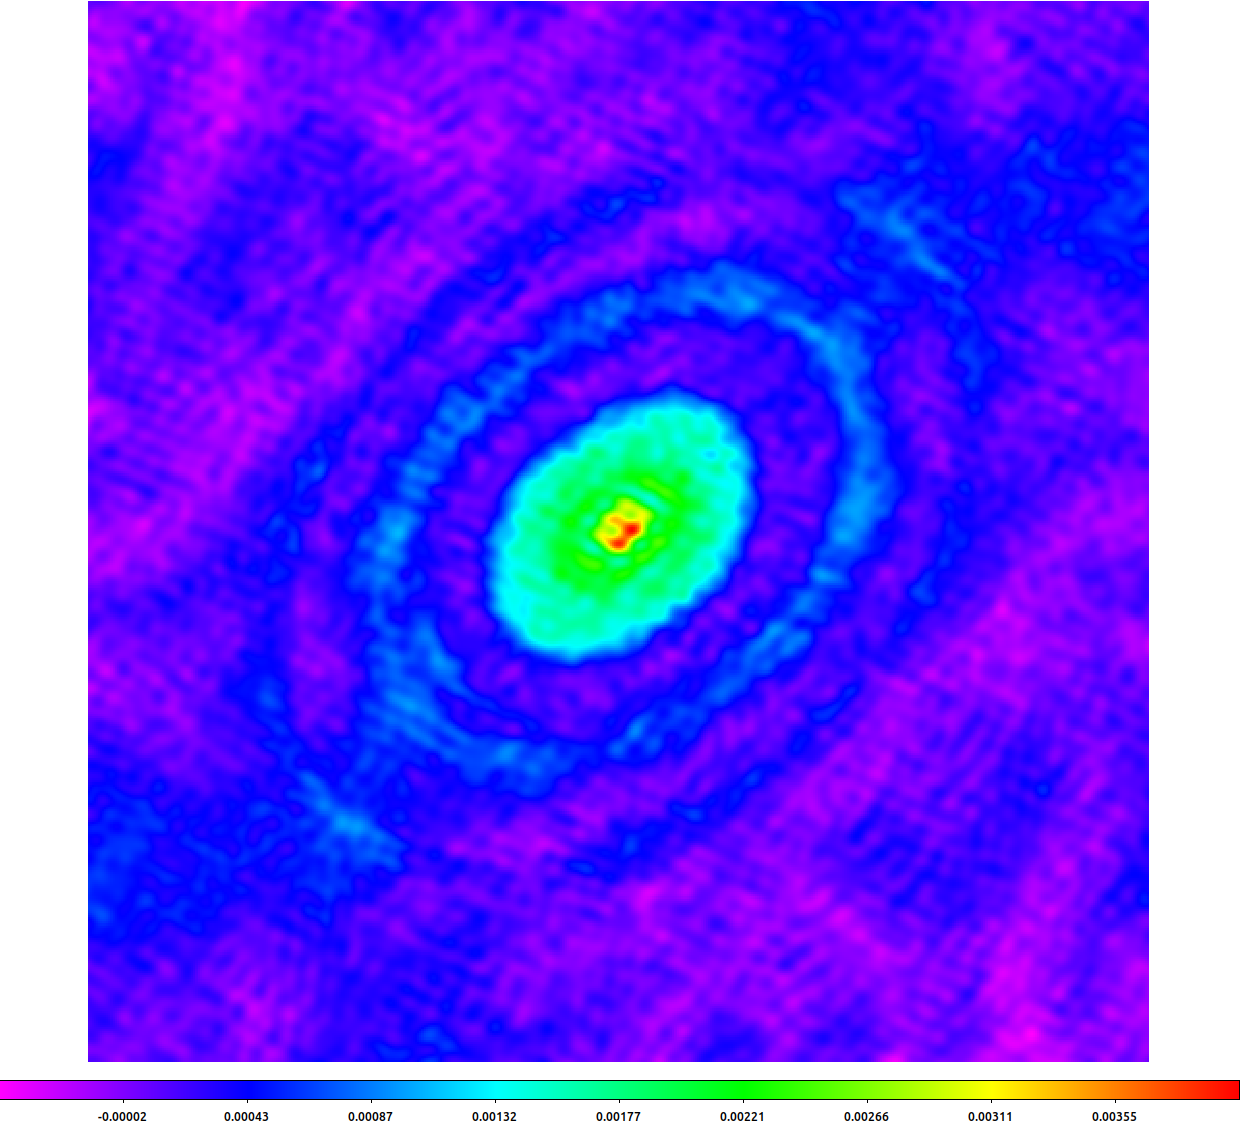
\includegraphics[width=0.45\textwidth]{images/HD163296_short8_colors.png}}
 \caption[Imagen sucia de HD163296 reducido (\textit{long-baseline})]{Imagen sucia de HD163296 reducido (\textit{long-baseline}). Fuente: Elaboración propia.}
 \label{fig:hd163296_obs8}
\end{figure}

\begin{figure}[!ht]
 \centering
  \subfloat[Colores originales]{
   \label{fig:short_base_original}
    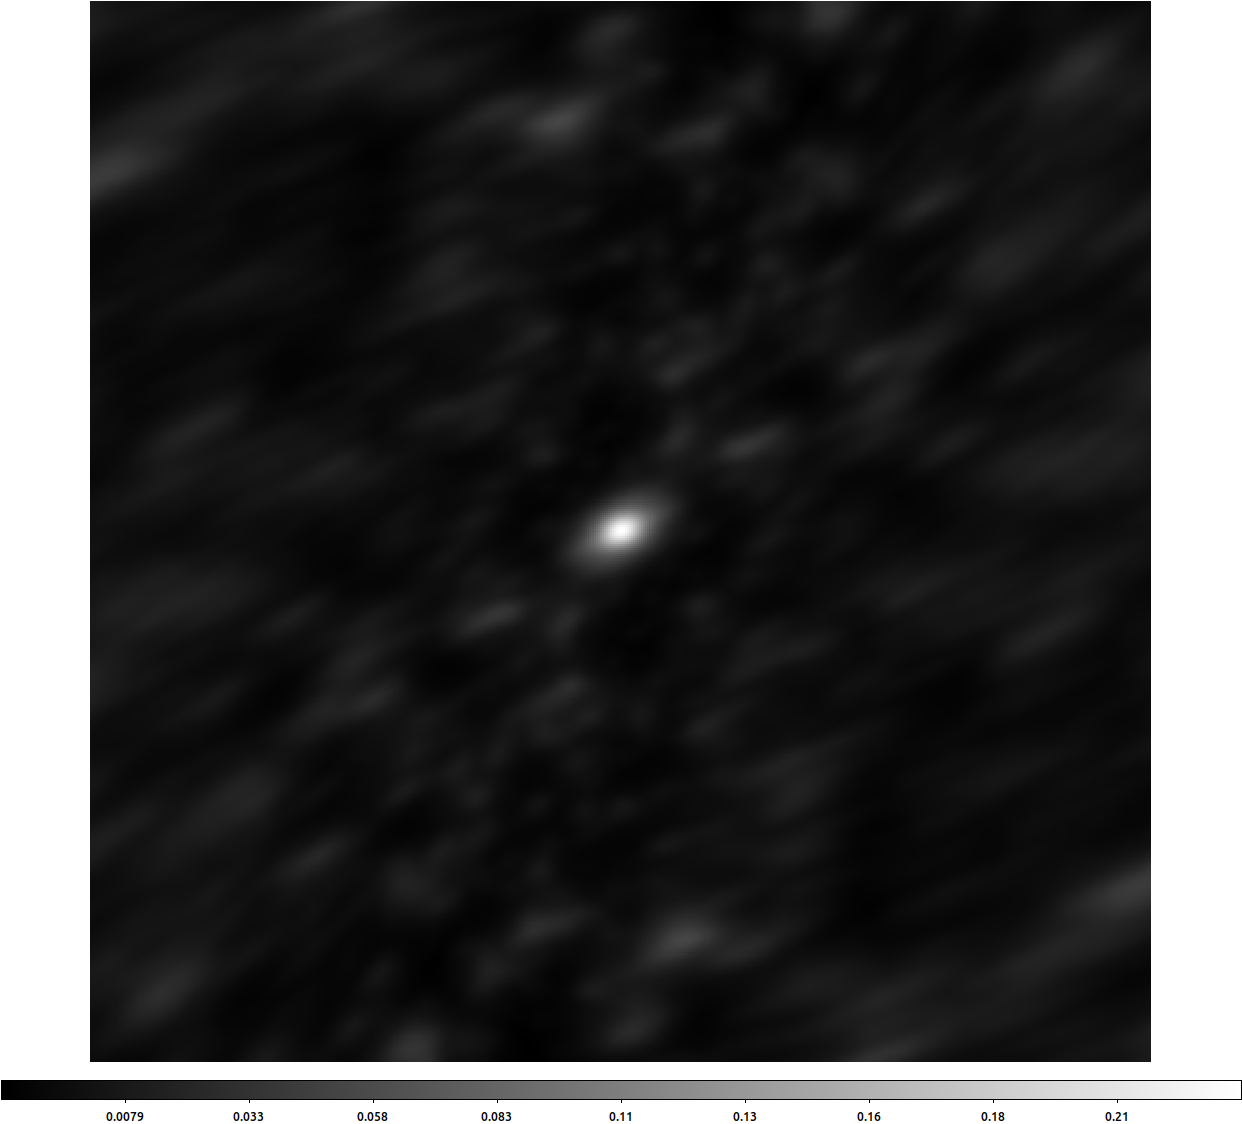
\includegraphics[width=0.45\textwidth]{images/short_base_obs3.png}}
  \subfloat[Colores artificiales]{
   \label{fig:short_base_color}
    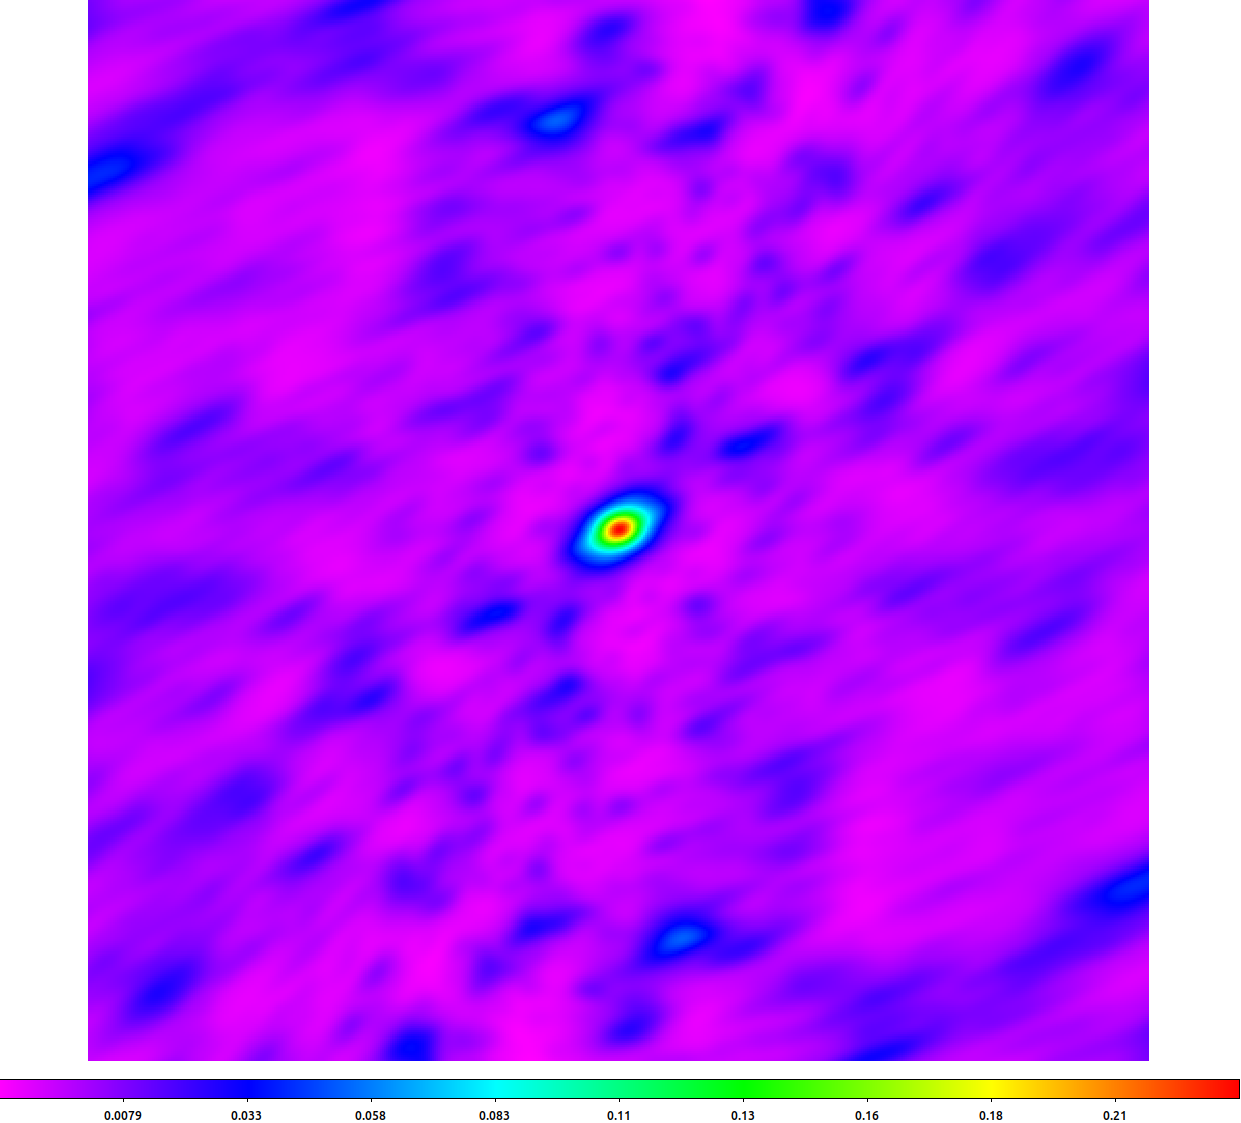
\includegraphics[width=0.45\textwidth]{images/short_base_obs3_color.png}}
 \caption[Imagen sucia de HD163296 reducido (\textit{short-baseline})]{Imagen sucia de HD163296 reducido (\textit{short-baseline}). Fuente: Elaboración propia.}
 \label{fig:hd163296_obs3}
\end{figure}


\subsection{Imagen artificial}
\label{subsec:artificial_image}

Una imagen de un objeto astronómico artificial es creada a través de un script en el lenguaje de programación \texttt{Python}. Esta imagen se encuentra en un formato FITS con un tamaño de 512x512 y será utilizada como si fuera el objeto a calibrar, es decir, como si fuera un objeto existente en el espacio exterior. La Figura \ref{fig:simulated_image} muestra la forma de este objeto donde cabe destacar que el \textit{header} de está imagen FITS es distinto según sea \textit{short-baseline} o \textit{long-baseline}. 

\begin{figure}[!ht]
	\centering
	\captionsetup{justification=centering}
	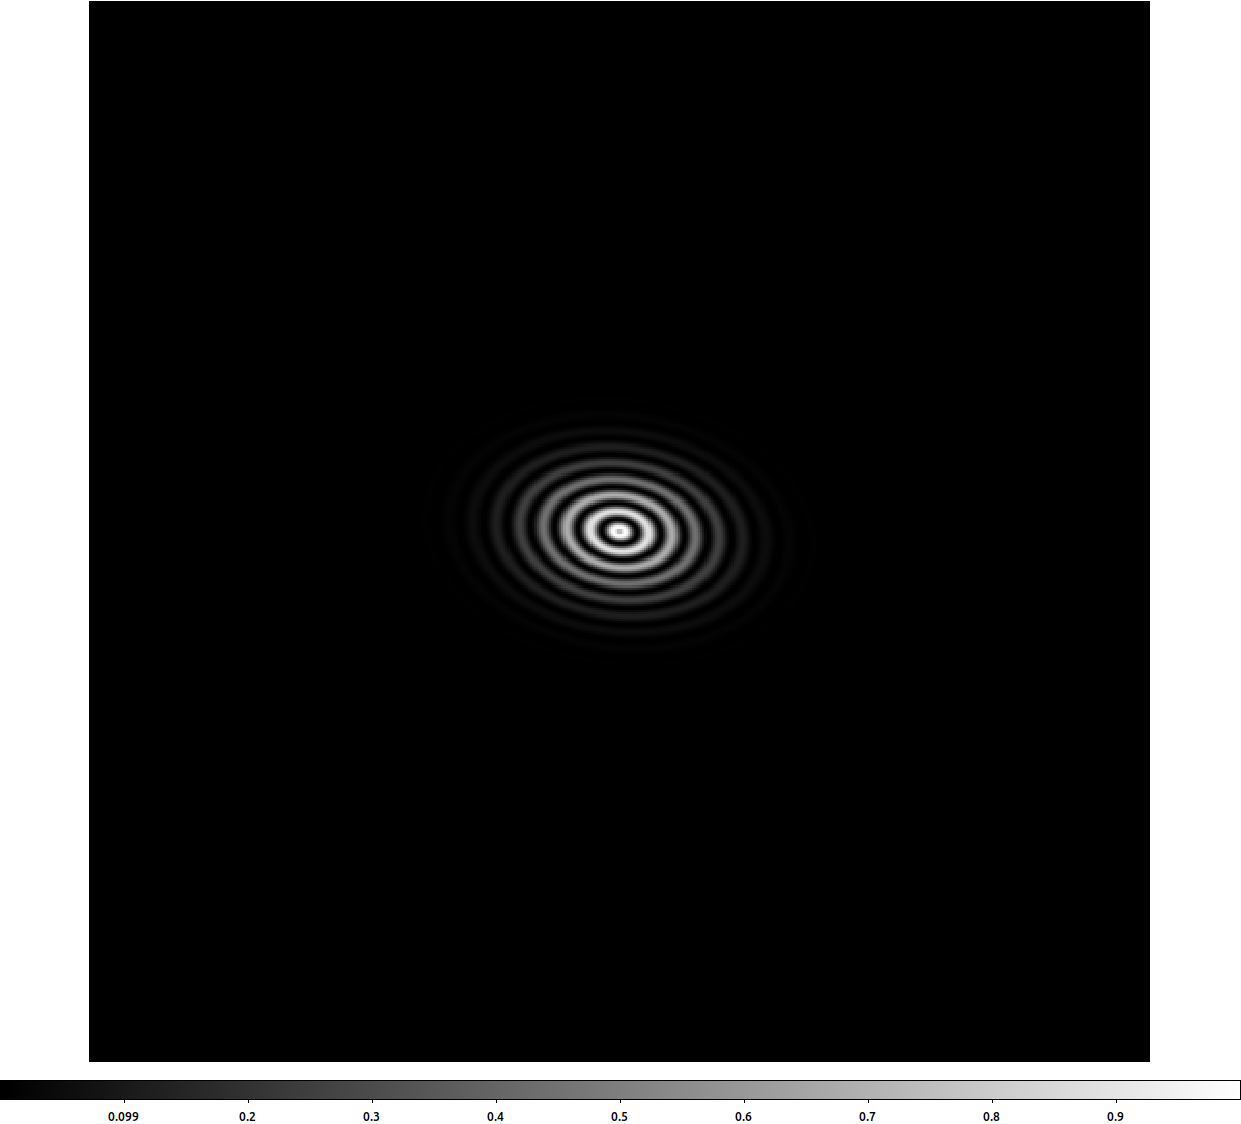
\includegraphics[scale=0.35]{images/simulated_image.png}
	\caption[Imagen artificial]{Imagen artificial. Fuente: Elaboración propia}
	\label{fig:simulated_image}
\end{figure}

\subsection{Conjunto de datos simulado}

Finalmente para crear el conjunto de datos simulado se necesita principalmente la imagen sucia creada en \ref{subsec:dirty_image} y la imagen artificial creada en \ref{subsec:artificial_image}. Obtenido esto se debe realizar los siguientes pasos. 

\begin{enumerate}
    \item Crear una imagen artificial, del tipo FITS, que contenga el \textit{Header} del conjunto de datos reducido de HD163296 y los datos de la imagen artificial. Este script puede ser visto en el Apéndice \ref{finales:apendice4}. 
    \item A través del comando \texttt{imporfits} del framework CASA, la imagen artificial anterior se convierte de su formato FITS a un formato Image. 
    \item Utilizando el comando \texttt{ft} del framework CASA se puede ingresar una columna modelo hacia un conjunto de datos. De esta manera la conjunto de datos reducido de HD163296 se le ingresa una columna modelo utilizando la imagen artificial en formato Image creada en el paso anterior. 
    \item Finalmente, la creación de un nuevo conjunto de datos puese ser lograda a través del comando \texttt{mstransform} del framework CASA. Este permite intercambiar la columna MODEL con la columna DATA, de tal manera de que la información de la imagen artificial sea la presente en el conjunto de datos creado. 
\end{enumerate}

De esta manera se obtiene un nuevo conjunto de datos que contiene visibilidades simuladas pero con la demás información como cantidad de antenas, tiempo de observación, pesos, entre otros, es parte del conjunto de datos reducido HD163296. Los comandos utilizados en los pasos 2,3 y 4, junto a los parámetros utilizados en estos pueden ser encontrados en el Apéndice \ref{finales:apendice5}. 